% ----------------------------------------------------------
% Fundamentação Teórica
% ----------------------------------------------------------
\chapter{Fundamentação Teórica}
\label{cha:fundamentacao}

Nesta seção apresenta o referencial teórico relacionado às peculiaridades necessárias para o desenvolvimento de um sistema web com seu objetivo. É importante destacar que esse modelo pode ser hospedado fora do ambiente físico da empresa, permitindo o acesso por usuários devidamente cadastrados. Dessa forma, o sistema pode ser utilizado enquanto houver uma conexão de internet adequada para sua operação.

\section{História da industrialização}
\label{sec:hist_industria}

A humanidade sempre buscou desenvolver ferramentas desde os primórdios com o objetivo de facilitar o trabalho e realizando manutenções conforme o necessário. É importante ressaltar que, ao longo do tempo, essas ferramentas rudimentares passaram por aperfeiçoamentos, resultando em utensílios mais específicos que visam aprimorar as atividades realizadas. No entanto, a precisão e a padronização só começaram a surgir a partir da Revolução Industrial.

De modo que a indústria encontra-se em sua quarta geração, conforme ilustrado na Figura \ref{fig:etapas_industria}. Assim, a manutenção deve estar sempre alinhada às atualizações da versão industrial, pois precisa fornecer o suporte técnico necessário para solucionar defeitos nos maquinários. A primeira versão de manutenção é conhecida como ``manutenção corretiva sem planejamento", onde as intervenções são limitadas a rotinas básicas, como a troca de peças com avarias por desgaste ou quebra, além de limpezas e lubrificações. Vale ressaltar que as máquinas só paravam quando apresentavam um defeito que as tornava inoperantes em realizar a atividade \mbox{\cite{a:manutencao_industriav4_2023}.}

\begin{figure}[th!]
    \centering
    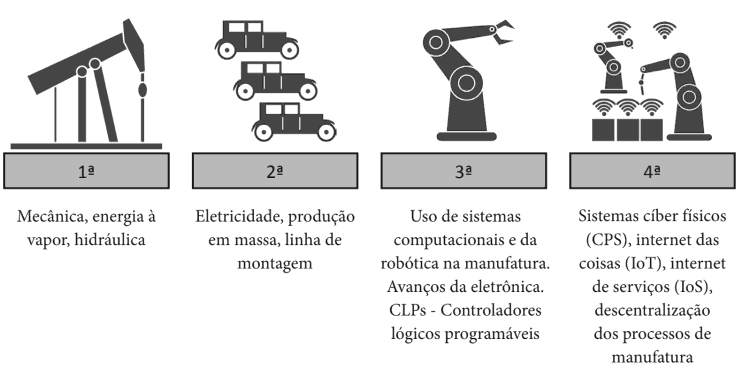
\includegraphics[width=0.75\linewidth]{figs/industria_as_4_versoes.png}
    \caption{Ilustração sobre as versões da indústria \cite{b:industria_v4_2018}}
    \label{fig:etapas_industria}
\end{figure}

A segunda fase concentrou-se na manutenção preventiva. Nesse contexto, surgiram os primeiros sistemas de planejamento e controle de manutenção, que se tornaram componentes essenciais da manutenção moderna, especialmente por razão das duas Guerras Mundiais. Muitas empresas implementaram planos de desenvolvimento na produção, impulsionadas pela necessidade de manter seus maquinários em condições aceitáveis para desempenhar suas funções. Além disso, as indústrias começaram a buscar maneiras de prolongar a vida útil de seus produtos, visando fidelizar os clientes em resposta ao aumento dos custos. Modelos como fordismo, toyotismo e taylorismo passaram a ganhar destaque.

 De acordo com a análise realizada por \mbox{\citeonline{a:manutencao_industriav4_2023},} a terceira fase da indústria pode ser caracterizada pelos seguintes tópicos.
 \begin{itemize}
     \item \textbf{Just-in-Time (JIT)}: Esse método contribui para a redução do desperdício e a melhoria da eficiência, assegurando que os materiais cheguem na hora e na quantidade adequadas, evitando excessos de estoque. Para isso, é essencial um planejamento logístico eficaz e uma colaboração estreita com os fornecedores, sendo os contratos fundamentais para a formalização dessa parceria.

     \item \textbf{Impactos da Paralisação}: As interrupções na cadeia de suprimentos podem impactar negativamente tanto a qualidade quanto os custos de produção. Ressaltando a importância de elaborar planos de contingência e estratégias eficazes de gerenciamento de riscos, a fim de evitar a perda de desempenho e garantir que as demandas planejadas sejam atendidas de maneira adequada.

     \item \textbf{Segurança}: A segurança é uma preocupação fundamental, e as empresas devem cumprir normas e legislações rigorosas que visam proteger os colaboradores. A adoção de práticas seguras não apenas promove um ambiente de trabalho mais protegido, mas também contribui para a melhoria da moral da equipe e eleva a produtividade.

     \item \textbf{Legislação Ambiental}: O aumento da atenção às questões ambientais tem impulsionado as organizações a adotar práticas sustentáveis, como a redução de resíduos e o uso eficiente dos recursos naturais. Essas iniciativas não apenas proporcionam benefícios econômicos, mas também melhoram a imagem corporativa das empresas na sociedade.

     \item \textbf{Informática na indústria}: A adoção de sistemas contribui para aumentar a confiabilidade na produção, permitindo a implementação de manutenção preditiva, que utiliza estatísticas para prever possíveis falhas. Com testes realizados sob supervisão, é possível obter métricas que indicam quando é necessária uma intervenção, minimizando assim o tempo de parada do maquinário.  
 \end{itemize}

A quarta versão da indústria pode ser caracterizada como uma atualização significativa da terceira. Durante a terceira versão, observou-se uma falha de comunicação entre os setores de engenharia, manutenção e operações, resultando em uma elevada taxa de produtos manufaturados com defeitos precoces. Nessa fase, a manutenção era tratada como um mecanismo reativo para corrigir falhas. Em contrapartida, a quarta versão da indústria propõe uma abordagem preventiva, visando minimizar ao máximo a ocorrência de problemas \mbox{\cite{a:manutencao_industriav4_2023}.} De modo, essa nova abordagem estimula o compartilhamento de soluções e estratégias para lidar com avarias, aproveitando os avanços em tecnologia da informação e utilização de redes, que promovem uma comunicação mais eficaz e segura \mbox{\cite{a:osi_tcpip_2024}.}

\section{Tipos de manutenções}
\label{sec:tipos_manutencao}

Está seção aborda as categorizações dos tipos de manutenções que o referencial teórico explora, conforme os seguintes itens:

\subsection{Manutenção corretiva planejada}
\label{sub:manutencao_corretiva_planejada}

Trata-se de manutenções corretivas planejada, nas quais existe uma métrica que mensura quanto tempo de operação que uma peça pode suportar antes de comprometer a integridade do grupo ou por completo do maquinário, enfatizando a necessidade de cuidados durante a operação. Nesse contexto, o objetivo é planejar paradas programadas do maquinário e monitorar quais operações e cargas foram aplicadas durante um determinado período de trabalho. Para isso, é adotado um agendamento prévio para a manutenção, que permite monitorar o grau de desgaste das peças e identificar quais reparos e substituições são necessários. É importante ressaltar que a perda total de um maquinário pode ocorrer se essas manutenções não forem realizadas corretamente.

\subsection{Manutenção corretiva não planejada}
\label{sub:manutencao_corretiva_nao_planejada}

Trata-se de manutenções que ocorrem devido a falhas imprevistas, sem um planejamento pré-estabelecido. Essas falhas podem resultar de descuidos ou do uso excessivo do maquinário em atividades ou ainda da utilização de peças que já apresentam desgaste. Esse tipo de manutenção gera uma série de desafios logísticos, uma vez que o problema pode demandar a aquisição de várias peças que talvez não estejam disponíveis para o reparo que será realizado.

\subsection{Manutenção preventiva}
\label{sub:manutencao_preventiva}

Trata-se de manutenções rotineiras que têm como objetivo monitorar os parâmetros e realizar pequenos ajustes, por exemplo verificar os níveis de água e óleo, completando-os quando estão abaixo do recomendado. Essas manutenções visam identificar irregularidades que, se não corrigidos, podem resultar em falhas graves. Além disso, não é necessário ser um especialista para realizar essas intervenções, pois elas estão sempre documentadas nos manuais de instruções do maquinário.

\subsection{Manutenção preditiva}
\label{sub:manutencao_preditiva}

Estes são tipos de manutenção que permitem a detecção antecipada de problemas, exigindo um olhar especializado para identificar situações que possam resultar em falhas futuras com uso software para analise de dados. A monitoração dos parâmetros de condição e desempenho dos equipamentos deve ser contínua, pois essas características são essenciais para prever o que pode ocorrer em determinadas circunstâncias. Conceito de sensores de falhas são implementados de modo primário.

\subsection{Manutenção prescritiva}
\label{sec:manutencao_prescritiva}

A manutenção prescritiva é uma evolução da manutenção preditiva. Esse método busca integrar ferramentas e sistemas da manutenção preditiva com técnicas de mineração de dados, utilizando algoritmos e modelos matemáticos para sugerir as melhores possibilidades de intervenção na manutenção. O objetivo é evitar paradas da máquina durante os períodos de maior demanda nas atividades de produção.

\section{Usinagem}
\label{sec:usinagem}

A usinagem é um processo fundamental na fabricação de peças, pois transforma insumos de diversos, como madeira, alumínio, nylon, aço e bronze, em produtos manufacturados. Esse processo utiliza ferramentas para remover o material em excesso, conhecido como desbaste, que gera cavacos, até que a peça atinja as dimensões desejadas do projeto, podendo em conjunto com outras peças formarem um equipamento por completo \mbox{\cite{a:guia_usinagem_2024}.}

Dessa forma, o torno é uma ferramenta que, embora simples, apresenta complexidade, pois opera em dois eixos: transversal e longitudinal conforme a Figura \ref{fig:tornos} contém um modelo mecânico manual e um computadorizado. Vale ressaltar para a operação desses maquinários é necessário utilizar API proteção individual como abafadores ruídos, óculos protetor ocular ou mascara protetora facial, luvas, roupas e botinas adequadas para operação.

\begin{figure}[tbh!]
    \centering
    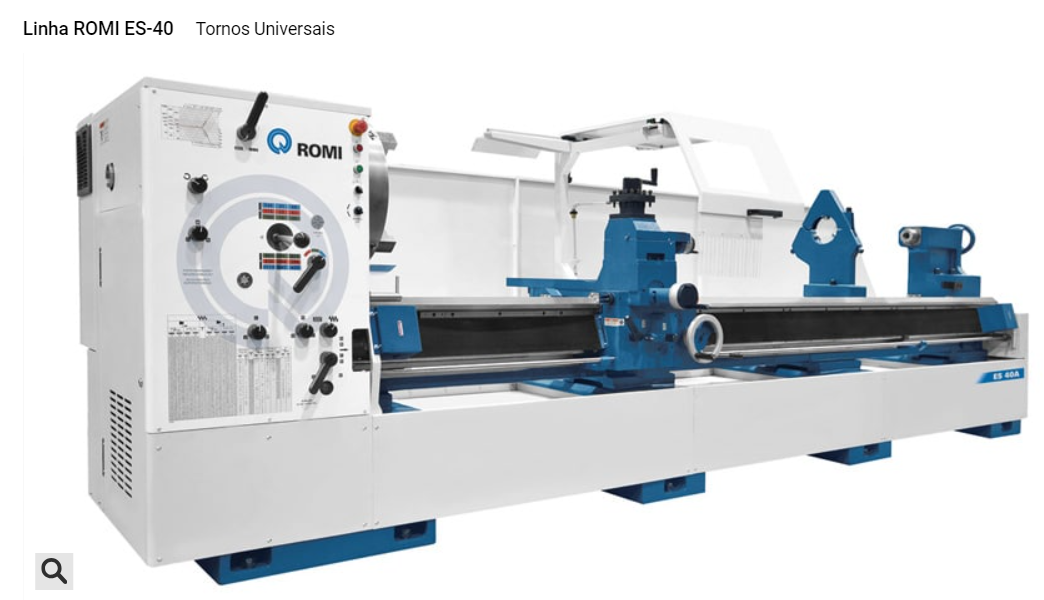
\includegraphics[width=0.48 \linewidth]{figs/rome_es40.png}
    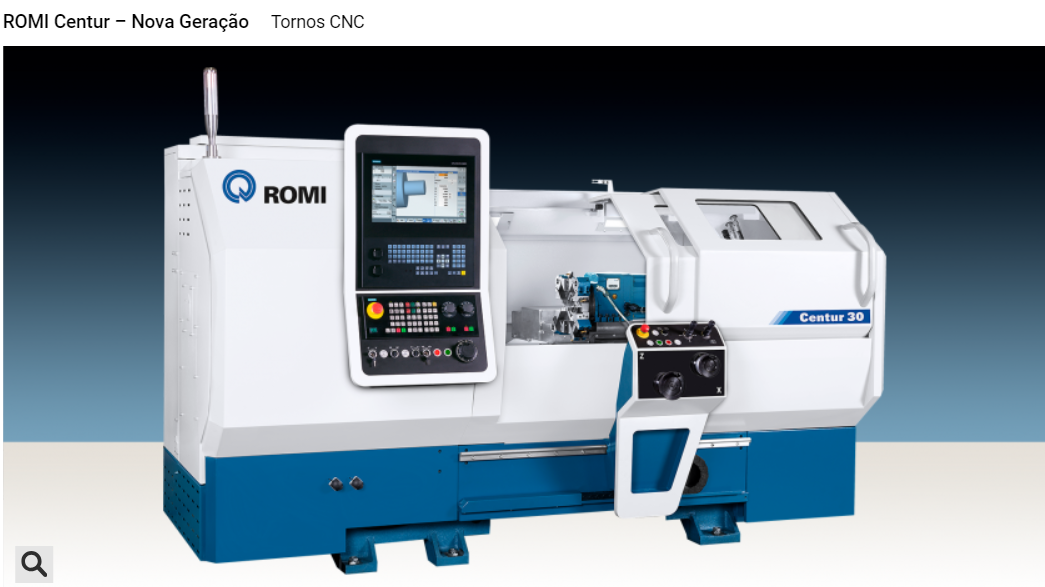
\includegraphics[width=0.48 \linewidth]{figs/romi_cnc.png}
    \caption{Imagem torno manual e CNC \cite{m:figs_tornos}}
    \label{fig:tornos}
\end{figure}

A Figura \ref{fig:tipo_usinagem} ilustra os principais métodos utilizados na manufatura na indústria, evidenciando que, muitas vezes, mais de uma atividade pode ser empregada para desenvolver uma determinada peça. Além disso, há peças que são inicialmente confeccionadas em formas, por meio de processos como estampagem ou fundição, e que posteriormente podem passar por acabamentos finais, como torneamento e fresamento.

\begin{figure}[h!]
    \centering
    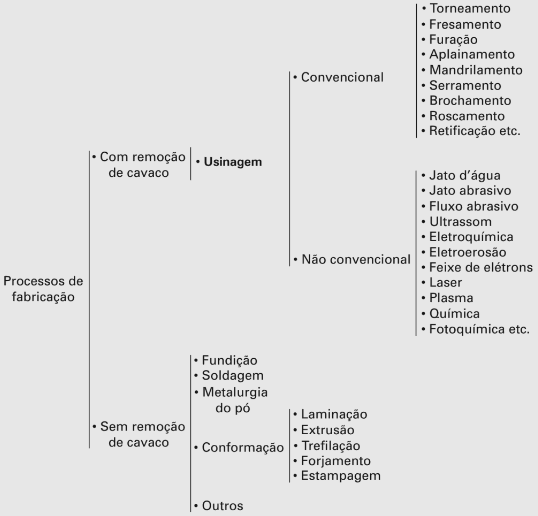
\includegraphics[width=0.75\linewidth]{figs/usinagem_tipos.png}
    \caption{Arvore fabricação de peças \cite{b:usinagem_2015} }
    \label{fig:tipo_usinagem}
\end{figure}

Graças à terceira revolução industrial, o sistema de usinagem avançou consideravelmente. Com o advento da informática, foi possível desenvolver tornos com comando numérico computadorizado, conhecidos como tornos CNC, conforme ilustrado Figura \ref{fig:tornos} imagem da direita. Para o desenvolvimento de peças, é fundamental criar um esquema de instruções, que pode ser elaborado por meio de softwares de \textit{Computer Aided Design  Computer Aided Manufacturing} (CAD-CAM) ou Solid-CAM na versão 3D, permitindo a criação do projeto da peça. Posteriormente, esses programas processa em esquema para a linguagem G-CODE, que é a linguagem padrão utilizada pelos tornos CNC para controlar todos os movimentos da máquina. Além disso, esses sistemas estão equipados com mecanismos de segurança que interrompem as operações em caso de falhas mecânicas, de hardware ou de software \mbox{\cite{a:torno_cnc_2022}.}

\section{Tecnologias para desenvolvimento web}
\label{sec:tecnologia_web}

Quando um usuário acessa um navegador e insere um endereço válido na internet, o navegador carrega um site específico, que, neste caso, corresponde a uma página ou sistema. Vários fatores estão envolvidos na determinação da página web a ser carregada, pois o processo se inicia com requisições de serviços. Essas requisições são essenciais para a comunicação entre o navegador e os servidores, permitindo que os dados sejam transferidos e a página desejada seja exibida ao usuário

Assim, para que máquinas e humanos, ou apenas máquinas, possam trocar informações, faz-se necessário a utilização de modelos e protocolos que padronizem o processo de envio e recebimento de dados. Nesse sentido, a web é constituída por um conjunto de pacotes organizados em uma estrutura hierárquica, que orienta os métodos de verificação para que não haja erros na transmissão. De modo que a comunicação, por sua vez, é realizada por meio de interfaces de programação, utilizando protocolos como o \textit{Hypertext Transfer Protocol} (HTTP), \textit{Hypertext Transfer Protocol Secure} (HTTPS) e \textit{File Transfer Protocol} (FTP), entre outros \mbox{\cite{b:redes_2017}.}

Por meio desses formatos e métodos, as páginas da web emprega \textit{Uniform Resource Locator} (URL), que converte \textit{World Wide Web} (WWW) em IP de domínios com o auxilio \textit{Domain Name System} (DNS) que realiza essa codificação. Assim, o navegador recebe esse endereço e o transmite para seus nós, realizando saltos através de roteadores que verificam quais rotas devem ser seguidas para levar a solicitação em menor tempo do cliente ao servidores e depois podem optar por rotas alternativas mais viáveis para retornar as solicitações \mbox{\cite{b:redes_2017}.}

Após estabelecer todos os mecanismos de comunicação necessários para a solicitação das informações, é essencial utilizar uma linguagem de marcação juntamente com uma linguagem de programação que contenha a lógica do sistema, permitindo o desenvolvimento do ambiente pode ser um site, blog ou um sistema web, havendo assim classificação como no back-end e front-end.

Dessa forma, o \textit{Hypertext Markup Language} (HTML) oferece a estrutura visual e esquemática essencial para que o usuário possa visualizar e interagir com o sistema, o HTML encontra se na sua quinta versão. Para aplicar estilizações, o \textit{Cascading Style Sheets} (CSS) proporciona melhorias visuais que formatam e facilitam a manutenção sempre que um elemento precisa de uma nova apresentação, de modo que framework mais utilizado é Bootstrap que está na sua quinta versão, que já contém uma estrutura estabelecidas basta conhecer a sintaxe para declara las nas tags do HTML. Por outro lado, para as máquinas, são suficientes conjuntos de protocolos, métodos, parâmetros e regras que organizam o envio e o recebimento das solicitações entre elas e o servidor, há bibliotecas ou APIs que possibilitam essa interação de trafego de dados na rede \mbox{\cite{a:api_redes_industria_v4_2024}.}

Para implementar a lógica e desenvolver métodos como \textbf{Create}, \textbf{Update} e \textbf{Delete}, é necessária uma linguagem de programação web, que podem ser da linguagem Java, PHP, Python, entre outras opções e atualmente há suporte para linguagem JavaScript que realiza função lógica para desenvolver sistema. Assim, dependendo dessa opção do desenvolvimento da programação, há frameworks que garantam uma estrutura padrão já implementadas com rotinas mais comuns. Para o PHP por exemplo pode ser Codeigniter.

O CodeIgniter é um framework para o desenvolvimento de aplicações web. O objetivo deste framework é agilizar o processo de desenvolvimento por meio de bibliotecas nativas, permitindo a integração de novas bibliotecas conforme necessário, utilizando o Composer. Ele é projetado para criar aplicações mais enxutas, com um menor tempo de configuração para iniciar um projeto, uma programação menos restritiva e a possibilidade de utilizar linhas de comando para o desenvolvimento \mbox{\cite{b:codeigniter4_2020}.}

A versão 4 do CodeIgniter introduziu o componente Spark, que facilita a criação de diversos elementos, incluindo a configuração do banco de dados — que, neste projeto, utilizará MySQL — até o desenvolvimento de controllers e models da aplicação. Para acessar mais informações, basta digitar o comando \textbf{php spark} no prompt de comando dentro do diretório da aplicação. Para detalhes adicionais e acesso à documentação, visite o site oficial do CodeIgniter \mbox{\cite{m:codeigniter4.5.4}.}